\begin{abstract}
Audio language models increasingly hear synthetic voices: accessibility users who speak through text-to-speech, agent-to-agent calls, and robocalls. At the same time, most audits of these models are built with synthetic speech, on the assumption that being synthetic changes nothing. Nobody has tested that assumption with the speaker and the words held fixed. We do. From 40 LibriSpeech readers we take 200 real utterances and build three matched versions of each: a zero-shot clone of the same speaker saying the same words, a neural-codec re-encoding of the real recording, and a stock synthetic voice saying the same words. Each of the 800 clips is sent to Gemini 3.6 Flash, Gemini 3.1 Pro, and an open-weight model with five tasks: transcribe, grade the reading, answer a content question, say whether the voice is real or AI-generated, and reply as a voice assistant. First, the clone is invisible to behaviour. Gemini Flash grades the clone within 0.005 points of the real recording on a 10-point scale (95\% interval $-0.16$ to $+0.16$ over 200 paired items), transcribes both at 3\% word error rate, and answers content questions at ceiling on both. Second, the codec re-encoding is not invisible: the same model grades it 0.31 points lower ($p = 3.5 \times 10^{-4}$, surviving multiple-comparison correction). The model reacts to artifacts, not to provenance, which reverses our pre-registered expectation that artifacts would explain less than half of a provenance effect. Third, asked directly, the models cannot tell. Balanced accuracy for real versus clone is 0.555 (Flash) and 0.54 (Pro), and both models call most genuine recordings synthetic (74.5\% and 90\%). Fourth, the implicit behavioural signal is no larger than the explicit one, so the pre-registered prediction that models discriminate provenance without being able to report it is not supported. Fifth, an open-weight model, Voxtral-Mini-3B, on 40 paired items, grades the clone 0.18 points lower (interval $-0.40$ to $+0.05$, $p = 0.19$) and calls every clip real, so the two families lean in opposite directions on the probe and the sign pattern we pre-registered (Gemini at or above real, open-weight below) appears in the point estimates but is not statistically established. For Gemini, the practice of auditing audio models with synthetic stimuli is validated at a resolution of about a sixth of a grade point; the artifact sensitivity, and the strong bias toward calling real speech synthetic, are the findings that need attention.
\end{abstract}

\section{Introduction}
\label{sec:intro}

A voice agent hears a caller and does something: transcribes, grades, answers, or replies. Increasingly the caller is not a person speaking directly. People who use augmentative communication devices speak through text-to-speech. Voice-banking users who have lost their voice speak through a clone of it. Agents call other agents. And a large share of unsolicited calls are synthetic: a 2026 honeypot study found at least 27\% of robocalls used generated voices \citep{a2609_11137}. Every deployed audio model therefore hears synthetic voices, and the working assumption is that it treats them the same as real ones.

The same assumption sits under the research literature. Audio-model bias audits need many voices saying the same words, and the cheap way to get them is text-to-speech. Of 21 recent audio-LLM bias and fairness audits we reviewed, 16 use synthetic stimuli only (Section~\ref{sec:known}). Three of them name the synthetic-stimulus assumption as an untested limitation. None tests it. The question is simple to state: holding the speaker and the words fixed, does an audio model behave differently toward a synthetic rendering than toward the real recording?

The evidence that exists is indirect and contradictory. When Audio MultiChallenge re-rendered its human-recorded turns with a stock TTS voice, text-output models scored 7.5\% higher on the synthetic version and audio-output models 2.5\% lower \citep{a2512_14865}. MedMosaic reports that Gemini models score a few points higher on an ElevenLabs subset while four open-weight models drop by more than 12 points \citep{a2605_00969}. VoiceBench reports that all models do better on synthetic data \citep{a2410_17196}. In each case the synthetic and real arms contain different speakers and often different items, so the comparison cannot separate provenance from content, speaker, and recording conditions.

We built the matched comparison. The design has four arms per utterance (Figure~\ref{fig:teaser}). REAL is the original recording. CLONE is a zero-shot clone of the same speaker saying the same words, made from a separate reference clip of that speaker. RESYNTH is the real recording passed through a neural audio codec, which adds codec-like artifacts while leaving provenance untouched. STOCK is a default synthetic voice saying the same words, which is synthetic but not this speaker. The contrast CLONE minus REAL is the provenance effect. RESYNTH minus REAL tells us how much of it re-encoding alone would produce. STOCK minus REAL separates "synthetic in general" from "a clone of this person". We ask each model five things about every clip and, separately, whether the clip is real or AI-generated, so that we can compare what the model does with what it can report.

\paragraph{Findings.}
\begin{enumerate}
\item \textbf{The clone is invisible to behaviour.} On 200 paired items, Gemini 3.6 Flash grades the clone 0.005 points above the real recording (95\% interval $-0.16$ to $+0.16$, 10-point scale), transcribes both at 2.7\% and 2.9\% word error rate, and answers content questions correctly on 99.5\% of both. The stock voice is graded 0.005 points below real. Gemini 3.1 Pro, on 60 items, grades the clone 0.35 points higher, an interval of $-0.90$ to $+1.46$ that includes zero (Section~\ref{sec:results-clone}).
\item \textbf{The codec is not invisible.} The same Flash model grades the re-encoded real recording 0.31 points lower ($p = 3.5\times10^{-4}$, $d_z = 0.25$, survives Benjamini-Hochberg over 49 tests), with no change in word error rate. This is a positive control: the design detects a third-of-a-point effect when one exists. It also reverses our pre-registered direction D2, which expected artifacts to explain less than half of a provenance effect. There is no provenance effect to explain, and the artifact effect stands alone (Section~\ref{sec:results-codec}).
\item \textbf{Asked directly, the models cannot tell, and they lean synthetic.} Balanced accuracy for real versus clone is 0.555 (Flash) and 0.54 (Pro). Flash calls 74.5\% of genuine recordings synthetic; Pro calls 90\% synthetic. The clone raises that share by 11 points on Flash, and so does the codec re-encoding (13.5 points); neither shift survives correction (Section~\ref{sec:results-probe}).
\item \textbf{No hidden sensitivity.} Our pre-registered headline direction D1 predicted that a model's own grades would separate real from clone better than its stated answer does. They do not: the grade-based discriminability is 0.50 (chance) against 0.555 for the stated answer on Flash, and 0.53 against 0.53 on Pro (Section~\ref{sec:results-probe}).
\item \textbf{The open-weight model leans the other way, weakly.} Voxtral-Mini-3B, on 40 paired items (one per reader), grades the clone $0.18$ points below the real recording (interval $-0.40$ to $+0.05$, $p = 0.19$, $d_z = -0.25$), and answers REAL for every clip in the probe. Its own grades separate real from clone at AUC 0.575 against 0.50 for its stated answer, a difference whose interval touches zero. The pre-registered sign pattern D3 is present in the point estimates across the three families and not established by the tests (Section~\ref{sec:results-open}).
\end{enumerate}

\begin{figure}[t]
\centering
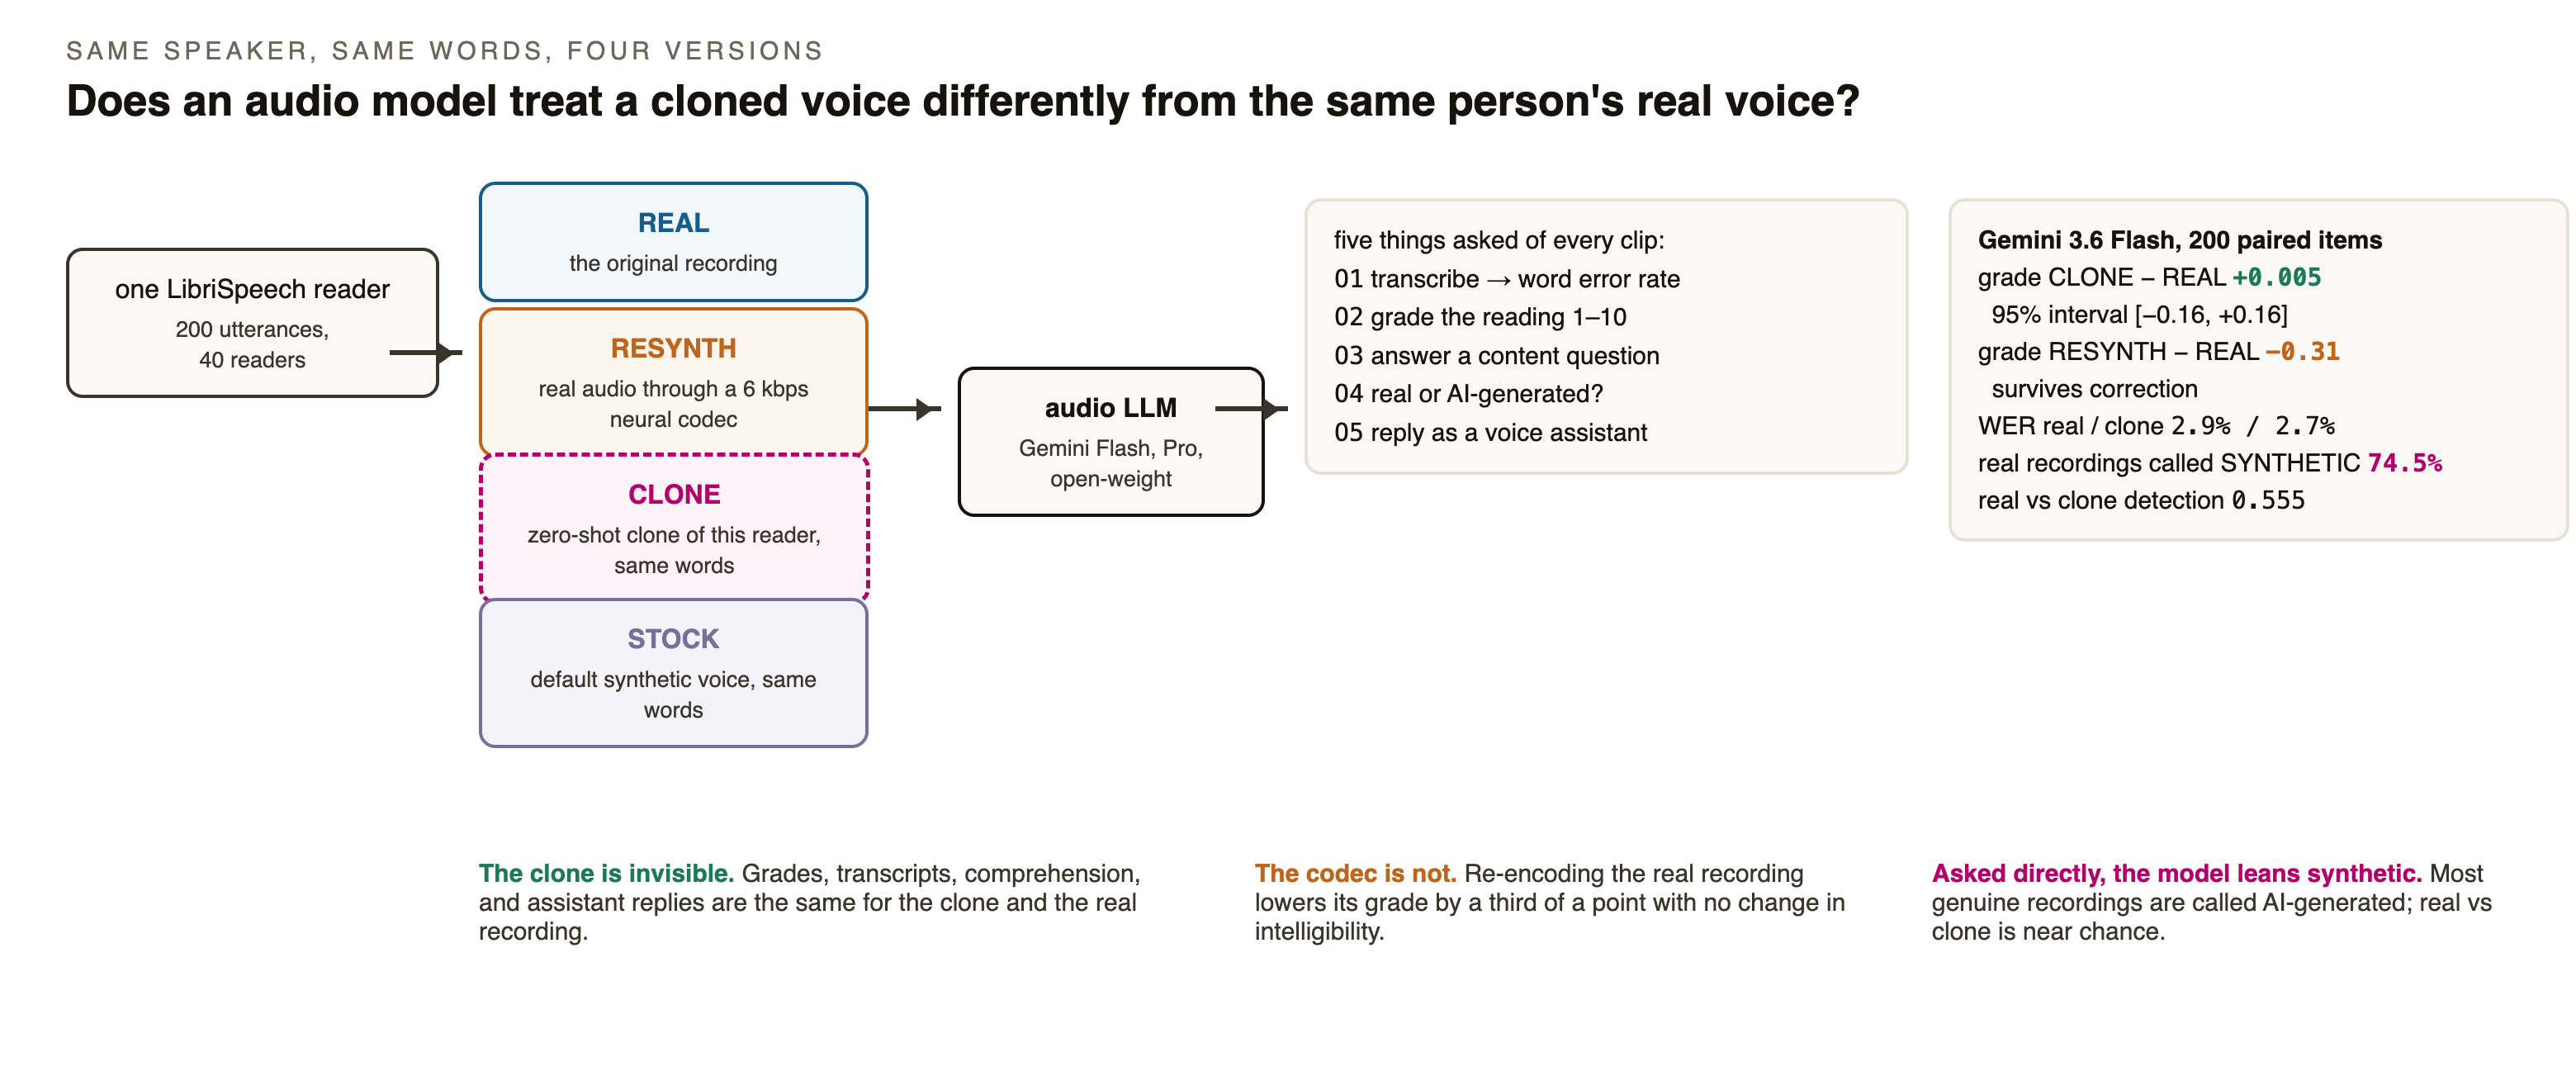
\includegraphics[width=\textwidth]{assets/fig1_teaser.png}
\caption{Study design and headline numbers. One real utterance becomes four clips (real, same-speaker clone, codec re-encoding, stock synthetic voice); each clip is graded, transcribed, questioned, probed for provenance, and answered as a voice assistant. The clone leaves every behavioural measure unchanged; the codec lowers the grade; the explicit probe is near chance with a strong bias toward calling real speech synthetic.}
\label{fig:teaser}
\end{figure}

\paragraph{What this means.} For the Gemini family, the synthetic-stimulus methodology that most audio-bias audits rely on is validated: a cloned voice produces the same grades, transcripts, comprehension, and assistant replies as the real one, to within about a sixth of a grade point. Two things still need attention. The models are sensitive to codec artifacts, so an audit whose synthetic arm carries more compression than its real arm will measure the codec, not the voice. And when asked, the models call most real speech synthetic, so any deployment that lets the model's own judgement of "is this a real person" gate a decision will fail real callers far more often than it catches synthetic ones.

\paragraph{Responsible framing.} Voices are cloned only from LibriSpeech, a public-domain audiobook corpus released under CC BY 4.0, only as matched stimuli, and are not released as voices. No deployed system was probed beyond public model APIs. The clone generator's audio watermark was disabled at generation so that the clone arm carries no signal the real arm lacks; the clips exist only for this measurement.

\section{What was known and what is new}
\label{sec:known}

We want to be clear about what is already known. That audio models cannot reliably say whether speech is synthetic when asked is established: zero-shot detection is at or below chance for Qwen-Audio \citep{a2505_11079} and "nearly at chance" for Gemini 2.5 Pro \citep{a2512_10652}, and GPT-4o refuses the question \citep{a2505_16211}; every detector that works is fine-tuned \citep{a2603_10725,a2601_00777}. That an audio model can encode an acoustic cue in its hidden states and act on it without reporting it is established for other cues \citep{a2605_13737,a2609_00727}. That synthetic subsets score differently from real ones is established and contradictory \citep{a2512_14865,a2605_00969,a2410_17196}. What is new here is the matched design, the resynthesis control, and the comparison of implicit against explicit sensitivity on the same clips.

\begin{table}[h]
\small
\centering
\begin{tabular}{p{4.2cm}p{9.0cm}}
\toprule
\textbf{Closest neighbour} & \textbf{What it established / what it does not cover} \\
\midrule
Audio MultiChallenge \citep{a2512_14865} & Human turns re-rendered with a stock TTS voice: text-output configs $+7.5\%$, audio-output configs $-2.5\%$. Different voice from the speaker; accuracy only; no probe; no codec control. \\
Counterfactual Audits \citep{a2608_06718} & Judge profiles on synthesised vs original audio agree at $\rho > 0.9$. Rank-order stability, no per-item delta, no detection outcome. \\
MedMosaic \citep{a2605_00969} & Real vs ElevenLabs subsets: Gemini $+1.4$ to $+3.3$, open-weight models $-12$ or worse. Unmatched subsets; a side-table. \\
VoiceBench \citep{a2410_17196} & "All models achieve better performance on synthetic data." Different items and speakers per arm. \\
BiasInEar \citep{a2602_01030} & Chatterbox clones of three real speakers used to validate stock-TTS bias patterns. The real recordings are never evaluated. \\
ALLM4ADD, TriDF, AudioTrust \citep{a2505_11079,a2512_10652,a2505_16211} & Explicit detection near chance, or refused. Detection only; no behavioural outcome on the same clips. \\
PhonemeDF \citep{a2603_15037} & Parallel real and synthetic LibriSpeech stimuli. Outcome is detector accuracy only. \\
\bottomrule
\end{tabular}
\caption{Novelty delineation. Full related work in Section~\ref{sec:related}.}
\label{tab:delineation}
\end{table}

\textbf{Ours alone.} (i) A matched speaker-and-content provenance treatment (REAL vs a zero-shot CLONE of the same utterance) with per-item paired statistics over 40 speakers. (ii) A neural-codec RESYNTH control and a STOCK arm that separate provenance from re-encoding and cloned identity from synthetic-in-general. (iii) Behavioural outcomes (grade, comprehension, assistant reply) plus transcription as the intelligibility covariate on every clip. (iv) The implicit-versus-explicit comparison: the model's own grade as a discriminator of provenance against its stated REAL/SYNTHETIC answer on the same pairs.

\textbf{Significance.} Who is affected: every deployed audio model that hears accessibility users, voice-banking users, agent-to-agent calls, or robocalls; and every audit built on synthetic stimuli, which is 16 of the 21 we reviewed. What changes: for the family we tested most fully, the synthetic-stimulus practice is validated to about 0.16 grade points, which is the first such number; audits must equalise codec and compression across arms, because the model reacts to those; and a model's own answer to "is this a real person" must not gate a decision, because it calls most real callers synthetic.

\section{Method}
\label{sec:method}

\textbf{Speakers and items.} LibriSpeech test-clean \citep{librispeech} has 40 readers (20 women, 20 men) with gold transcripts. For each reader we select, with a fixed seed, five target utterances of 4 to 12 seconds and 10 to 40 words, and one reference utterance of 5 to 10 seconds, disjoint from the targets, for cloning. Ten readers get a second reference for a stability battery. This gives 200 items. Mean item duration is 7.6 seconds.

\textbf{Four arms.} REAL is the original 16 kHz recording. CLONE is generated by Chatterbox \citep{chatterbox}, an open zero-shot cloning model, from the reader's reference clip and the target's gold transcript, with default settings and a fixed seed per item. RESYNTH is the real recording passed through EnCodec at 24 kHz and 6 kbps \citep{a2210_13438}, then resampled to 16 kHz; it keeps the real waveform's provenance and adds neural-codec artifacts. STOCK is Chatterbox's built-in default voice reading the same transcript: synthetic, but not this speaker. All 850 clips (800 plus 50 second-reference clones) are loudness-normalised to $-23$ LUFS, padded with 0.2 s of silence, and frozen with a SHA-256 manifest before any model call. Chatterbox normally embeds a watermark in its output; we disabled the watermarker at generation so that CLONE and STOCK carry no signal that REAL and RESYNTH lack. Clone and stock clips are on average 0.8 s shorter than the real ones (6.7 s vs 7.6 s), which we report as a known difference.

\textbf{Models.} Gemini 3.6 Flash runs the full grid (800 clips, five outcomes, plus batteries). Gemini 3.1 Pro runs a subset of 20 readers, three items each, four arms (240 clips) on three outcomes. Both are called through OpenRouter at temperature 0 with minimal reasoning, one clip per call in randomised order. Voxtral-Mini-3B-2507 \citep{a2507_13264}, an open-weight audio model, runs locally in bfloat16 on CPU (its audio encoder crashed on the Apple GPU), greedy decoding, on a reduced grid of 40 readers, one item each, REAL and CLONE arms, for the grade and the probe (159 calls at about 65 seconds each), because a cloud GPU was not available to us on the day. Other hosted audio families were unavailable to us at the time of the study.

\textbf{Five outcomes.} Verbatim prompts are in Appendix~\ref{app:prompts}. O1 TRANSCRIBE: word error rate against the gold transcript after lowercasing and punctuation removal. O2 GRADE: as an examiner, rate the reading's clarity and fluency from 1 to 10, integer only. O3 COMPREHEND: a four-option content question about the passage, generated once per item from the gold transcript by a text-only model and shuffled with a fixed seed, answered from the audio. O4 PROBE: "Is this a real human recording or AI-generated speech? Answer REAL or SYNTHETIC." O5 ASSIST: reply to the caller as a phone voice assistant in two or three sentences; a text-only judge, blind to provenance, flags refusal, remarks on the voice, and requests to verify the caller, and we count words.

\textbf{Analysis.} The unit is the item. For each outcome we form paired within-item differences CLONE$-$REAL, RESYNTH$-$REAL, STOCK$-$REAL, and CLONE$-$RESYNTH. Tests are two-sided sign-flip permutation tests that flip whole speakers (20,000 permutations); intervals are 95\% bootstrap intervals over speakers (10,000 resamples); effect sizes are paired $d_z$. Direction D1 is tested by comparing two discriminabilities on the same items: the probability that the model's grade ranks the real clip above its clone (implicit), against the probability that the probe calls the clone synthetic and the real clip real (explicit), each an AUC with chance at 0.5. Benjamini-Hochberg correction runs over all 49 reported tests; only survivors are bolded. Every number in this paper is produced by one script from the raw logs.

\textbf{Pre-registration.} Five directions were recorded before any clip was cloned. D1: some family's implicit provenance delta exceeds its explicit detection. D2: the resynthesis control explains less than half of the clone effect. D3: sign differs by family, Gemini at or above real, open-weight below. D4: explicit detection under 60\% for every family. D5: word error rate does not differ between real and clone. We report each outcome in Section~\ref{sec:prereg}.

\textbf{Cost.} 6,420 hosted calls for \$2.99 in metered spend, plus about five hours of local compute for cloning and the open-weight model. Total spend is in Appendix~\ref{app:cost}.

\section{Results}

\subsection{The clone is invisible to behaviour}
\label{sec:results-clone}

Table~\ref{tab:main} gives every outcome by arm, and Figure~\ref{fig:grade} shows the grades and the paired deltas. Gemini 3.6 Flash grades the real recordings at 9.01 on average and the clones at 9.01. The paired difference is $+0.005$ points with a 95\% interval from $-0.155$ to $+0.161$ ($p = 1.0$, $d_z = 0.00$, $n = 200$). The stock voice is graded 8.995, a difference of $-0.005$ ($p = 1.0$). So neither being synthetic in general nor being a clone of this particular reader moves the grade; the STOCK and CLONE arms are indistinguishable from each other and from REAL. Transcription does not move either: word error rate is 2.9\% on real and 2.7\% on clone ($p = 0.87$), and 2.4\% on stock. The content question is answered correctly on 99.5\% of real and clone clips, which is a ceiling and tells us only that the clones are fully intelligible. The assistant replies are the same length (30.5 vs 30.7 words), refuse at the same rate (1.5\% vs 1.0\%), and never ask the caller to verify they are human. The judge flagged a remark about the voice in 1.5\% of real and 5\% of clone replies; a hand audit of 24 replies found every flag was the model noting that the caller seemed to be reading from a book, not a remark about the voice (Appendix~\ref{app:audit}).

Gemini 3.1 Pro, on 60 items, grades real at 8.24 and clone at 8.59, a difference of $+0.35$ with an interval from $-0.90$ to $+1.46$ ($p = 0.60$). Its comprehension is 100\% on every arm. The interval is wide because Pro's grades vary more across repeated calls than Flash's; it includes zero and it includes the Flash estimate.

\begin{table}[t]
\small
\centering
\begin{tabular}{llcccc}
\toprule
Model & Outcome & REAL & CLONE & RESYNTH & STOCK \\
\midrule
Gemini 3.6 Flash ($n{=}200$) & O2 grade (1--10) & 9.01 & 9.01 & \textbf{8.69} & 9.00 \\
 & O1 word error rate & .029 & .027 & .031 & .024 \\
 & O3 comprehension & .995 & .995 & .990 & 1.00 \\
 & O4 share called SYNTHETIC & .745 & .855 & .880 & .845 \\
 & O5 reply words & 30.5 & 30.7 & 30.8 & 31.2 \\
 & O5 refusal / voice remark & .015 / .015 & .010 / .050 & .015 / .025 & .005 / .020 \\
\midrule
Gemini 3.1 Pro ($n{=}60$) & O2 grade & 8.24 & 8.59 & 8.36 & 8.59 \\
 & O3 comprehension & 1.00 & 1.00 & 1.00 & 1.00 \\
 & O4 share called SYNTHETIC & .898 & .978 & .960 & .956 \\
\midrule
Voxtral-Mini-3B ($n{=}40$) & O2 grade & 8.48 & 8.30 & --- & --- \\
 & O4 share called SYNTHETIC & .000 & .000 & --- & --- \\
\bottomrule
\end{tabular}
\caption{Every outcome by provenance arm. Bold: the paired difference against REAL survives Benjamini-Hochberg over all 45 tests. Paired deltas with intervals are in Appendix~\ref{app:tables}.}
\label{tab:main}
\end{table}

\begin{figure}[t]
\centering
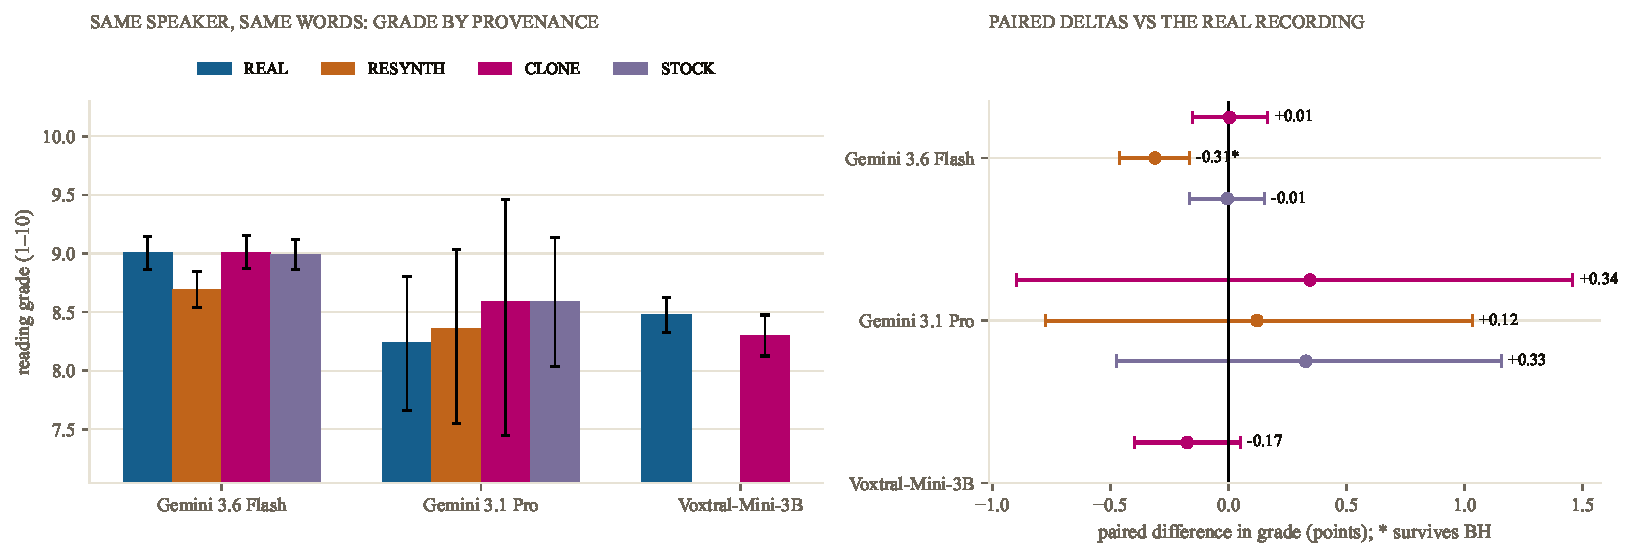
\includegraphics[width=\textwidth]{assets/fig2_grade.pdf}
\caption{\textbf{Left:} reading grade by arm and family, with 95\% speaker-bootstrap intervals. \textbf{Right:} paired differences against the real recording; a star marks a difference that survives correction. The clone and the stock voice sit on zero; the codec re-encoding does not.}
\label{fig:grade}
\end{figure}

\subsection{The codec is not invisible}
\label{sec:results-codec}

The RESYNTH arm is the same real waveform after a 6 kbps neural-codec round trip. Flash grades it 8.69, which is $-0.312$ points against real (interval $-0.460$ to $-0.162$, $p = 3.5\times10^{-4}$, $d_z = -0.25$, $n = 200$) and $-0.320$ against the clone ($p = 4.5\times10^{-4}$). Both differences survive correction; they are the only two of the 49 tests that do. Word error rate on RESYNTH is 3.1\%, not different from real ($p = 0.86$), and comprehension is 99\%. So the codec lowers the grade without lowering intelligibility.

This result does two jobs. It is a positive control: the paired design with 200 items detects a third-of-a-point shift, so the absence of a clone effect is not a lack of power. And it reverses our pre-registered direction D2. We expected a provenance effect and asked how much of it re-encoding alone would explain. Instead there is no provenance effect, and re-encoding produces an effect of its own. The model is reacting to something in the signal, and a state-of-the-art clone does not carry it while a 6 kbps codec does. On Pro the RESYNTH difference is $+0.12$ ($p = 0.81$) at $n = 60$; we cannot say whether the codec effect is Flash-specific or below Pro's resolution at this sample size.

\subsection{Asked directly, the models cannot tell, and they lean synthetic}
\label{sec:results-probe}

Figure~\ref{fig:probe} (left) shows the share of clips each model calls SYNTHETIC. Flash calls 74.5\% of the real recordings synthetic. It calls 85.5\% of clones, 88.0\% of codec re-encodings, and 84.5\% of stock-voice clips synthetic. Balanced accuracy for real against clone is 0.555; against stock it is 0.55. Pro is more extreme: 89.8\% of real recordings called synthetic, 97.8\% of clones, balanced accuracy 0.54. The clone raises Flash's synthetic share by 11.0 points (interval 3.0 to 19.0, $p = 0.015$) and the codec raises it by 13.5 points ($p = 0.0085$); neither survives correction, and the two are indistinguishable from each other ($p = 0.48$). Whatever the model uses to answer the question, it responds to re-encoding at least as strongly as to cloning, and it is dominated by a prior that speech is synthetic.

Direction D1 predicted that the model's behaviour would separate real from clone better than its answer does. Figure~\ref{fig:probe} (right) shows the two discriminabilities on the same items. On Flash the grade-based AUC is 0.503, which is chance, and the probe-based AUC is 0.555; the difference is $-0.05$ (interval $-0.08$ to $+0.02$). On Pro both are 0.53 (difference $-0.002$). The comprehension-based AUC is 0.50 on both. There is no hidden sensitivity: what little the models can discriminate, they can also say.

\begin{figure}[t]
\centering
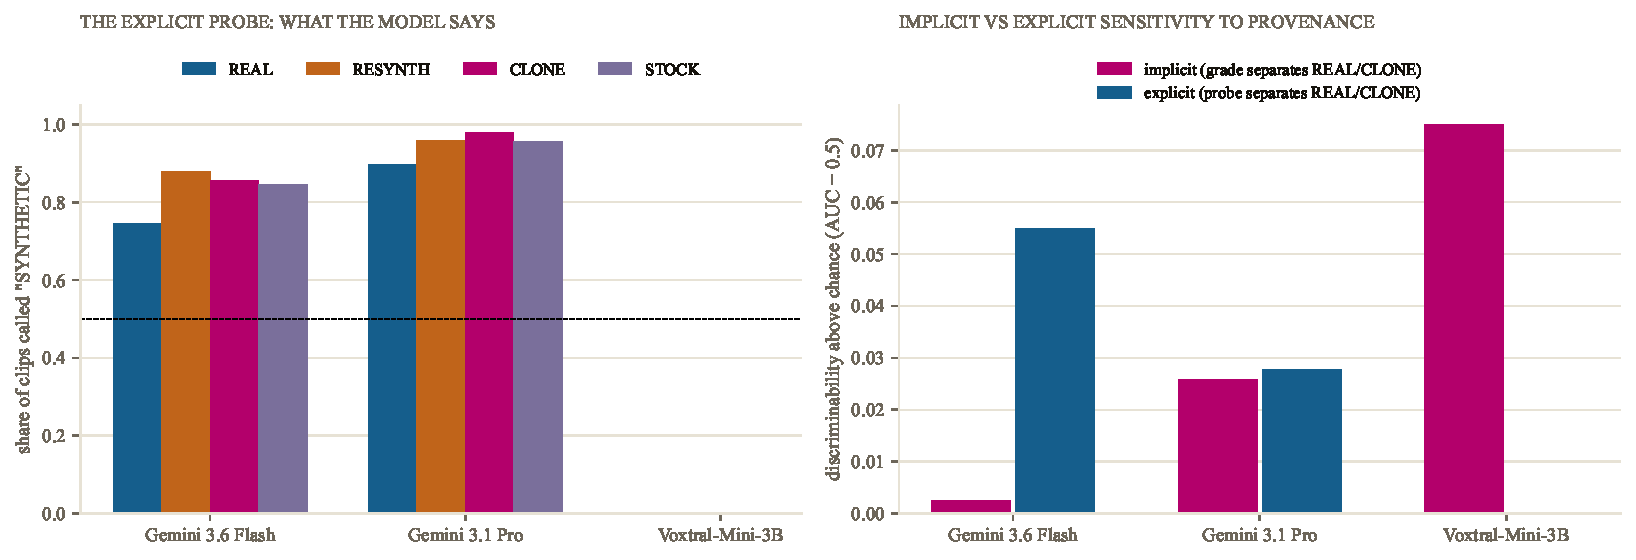
\includegraphics[width=\textwidth]{assets/fig3_probe.pdf}
\caption{\textbf{Left:} share of clips called SYNTHETIC by arm. Most real recordings are called synthetic. \textbf{Right:} discriminability of real from clone above chance, from the model's own grades (implicit) and from its stated answer (explicit). Neither is far from zero, and the implicit signal is not larger.}
\label{fig:probe}
\end{figure}

\subsection{The open-weight model leans the other way, weakly}
\label{sec:results-open}
Voxtral-Mini-3B grades the real recordings at 8.48 and the clones at 8.30 on the 40-item real-versus-clone subset. The paired difference is $-0.175$ points (interval $-0.40$ to $+0.05$, $p = 0.19$, $d_z = -0.25$, $n = 40$). The direction matches what MedMosaic reported for open-weight models and what we pre-registered as D3; the size is small and the interval includes zero. Asked whether each clip is real or AI-generated, Voxtral answers REAL for all 79 parsed clips, real and clone alike: balanced accuracy 0.50, the mirror image of Gemini's synthetic bias. Its own grades separate real from clone at AUC 0.575 (the clone is graded lower on more items than not), against 0.50 for the stated answer; the difference is $+0.075$ with a bootstrap interval from $0.00$ to $+0.175$. This is the one place in the study where the pre-registered pattern of D1, behaviour more sensitive than report, appears, and the interval's lower bound sits on zero, so we report it as suggestive and not as established. The family-by-provenance differences (Flash minus Voxtral $+0.18$, $p = 0.45$; Pro minus Voxtral $+0.65$, $p = 0.44$) do not reach significance at these sample sizes.

\subsection{Batteries: noise floor and clone stability}
\label{sec:results-batteries}

Thirty items were re-run five times each on Flash for the grade and the probe, at temperature 0. The grade changed across the five identical calls in 83\% of cells, with a mean within-cell standard deviation of 0.57 points; the probe answer flipped in 37\% of cells. The headline clone effect ($+0.005$) sits far inside this floor, which is the correct reading: the design averages 200 items, and the interval $\pm 0.16$ is the resolution of the average, not of one call. The codec effect ($-0.31$) is about half of one call's standard deviation and is established by pairing, not by any single cell.

For ten readers we cloned every target twice from two different reference clips. The grade differs between the two clones by 0.64 points on average in absolute value, with a signed mean of $-0.28$; the probe answer differs on 38\% of items. Clone-to-clone variation is therefore about the size of the codec effect and four times the clone-versus-real difference. A single clone per speaker, which is what most TTS-stimulus audits use, carries this much sampling noise.

\subsection{Pre-registered directions, scored}
\label{sec:prereg}

D1 (implicit exceeds explicit): not supported on either Gemini model. D2 (resynthesis explains under half of the clone effect): reversed; the clone effect is zero and the resynthesis effect is the only one present. D3 (sign differs by family, Gemini at or above real): the Gemini half holds, with clone at or slightly above real on both tiers; the open-weight point estimate is below real ($-0.175$), so the sign pattern is present, but no family-by-provenance difference is significant, so D3 is present in the point estimates and not established. D4 (explicit detection under 60\%): holds, at 0.555 and 0.54. D5 (word error rate equal): holds, 2.7\% against 2.9\%, $p = 0.87$.

\section{Limitations, narrated}
\label{sec:limitations}

The clones are good. Word error rate on CLONE equals REAL and comprehension is at ceiling, so our result is about high-quality zero-shot clones, not about synthetic speech in general. A worse synthesiser would sit somewhere between CLONE and RESYNTH, and our codec result says the model would react to it. Chatterbox's training data is undisclosed and LibriSpeech readers appear in public TTS training sets, so the clones may be of speakers the cloner has seen; that would make them better clones, which strengthens the null on behaviour but limits what we can say about unseen speakers.

The passages are audiobook sentences. The assistant task (O5) asks the model to reply to a caller who is reading a book, which is an odd call, and the replies mostly ask what the caller wants. That is why O5 shows nothing; it may also be why. A task with request-shaped content would be a better test of assistant behaviour, but it cannot be matched to real recordings of the same words without recording them.

Comprehension is at ceiling on every arm, so O3 cannot show a difference. It serves only as an intelligibility check. The grade is also near its ceiling (means of 9.0 on a 10-point scale for Flash), which compresses the range in which a penalty could appear. Two facts bound that concern: the codec penalty of 0.31 points is visible in the same compressed range, and Pro, whose grades sit lower (8.2 to 8.6), shows no clone penalty either. A harder grading task with lower baseline scores would still be a stronger test.

The grade noise floor is large: 83\% of cells change across identical calls at temperature 0. Our paired averages are precise to about a sixth of a point over 200 items, and every claim is scoped to that. Single-call comparisons in this setting would be uninterpretable.

Gemini 3.1 Pro ran 60 items, not 200, because of cost; its intervals are three times wider. The open-weight model ran on 40 items, one per reader, for two outcomes only, because it had to run on a CPU; its intervals are wide, and a full open-weight grid on a GPU is the obvious next step. Two hosted audio families we intended to test were unavailable to us at the time of the study.

The explicit probe is one wording. Models refuse or hedge less with a forced binary answer, which is why we used it, but the strong synthetic bias could be partly a property of the wording. We report the bias as a property of this prompt on these models.

\section{Related work}
\label{sec:related}

\textbf{Synthetic stimuli in audio-model audits.} FairDialogue, BiasInEar, MedVoiceBias, and The Voice Behind the Words generate their speaker variation with TTS or cloning and never evaluate the real recordings \citep{a2510_02352,a2602_01030,a2511_06592,a2603_16941}; VIBE and RedVox build real-speech benchmarks in explicit reaction to that practice \citep{a2604_17248,a2606_26968}; HumDial-EIBench critiques TTS benchmarks without running the comparison \citep{a2604_11594}. Several papers name the assumption as a limitation \citep{a2509_22061,a2604_14548,a2602_04796}. The judge literature reports that audio judges are robust to additive noise \citep{a2507_12705} and vulnerable to protocol shortcuts \citep{a2607_13477}; ParaPairAudioBench uses same-transcript pairs to expose judge calibration failures \citep{a2606_24648}.

\textbf{What audio models know about synthetic speech.} Zero-shot detection is near chance \citep{a2505_11079,a2512_10652,a2601_00777}, GPT-4o refuses \citep{a2505_16211}, and working detectors are trained \citep{a2603_10725}. Humans detect deepfakes at about 73\% \citep{mueller2021} and increasingly misjudge real speech as synthetic \citep{a2605_26136}. Hidden-state studies show audio models encode cues they do not report \citep{a2605_13737,a2609_00727}; verbal confidence from audio models is unreliable \citep{a2604_25591}, and yes/no bias is a documented failure mode \citep{a2604_19300}.

\textbf{Cloning, codecs, and robustness.} Zero-shot cloners report human-parity similarity on LibriSpeech test-clean with the same reference protocol we use \citep{a2410_06885,a2412_10117,a2605_30748}. Neural codecs and their artifacts are the basis of codec-fake detection \citep{a2210_13438,a2501_08238}. Audio-model robustness work finds that enhancement and compression change model behaviour in ways that quality metrics do not predict \citep{a2601_10384,a2608_30348,a2604_21276}, which is consistent with our codec result.

\textbf{Deployment stakes.} Synthetic voices are now common in unsolicited calls \citep{a2609_11137}, humans trust them differently \citep{a2605_28064,cambre2020}, and voice-banking and augmentative communication users depend on them daily.

\section{Conclusion}

We held the speaker and the words fixed and asked whether an audio model behaves differently toward a clone than toward the real recording. For Gemini 3.6 Flash the answer is no, to within a sixth of a grade point over 200 paired items, with identical transcription, comprehension, and assistant behaviour; Gemini 3.1 Pro agrees within its wider interval. An open-weight model, on a smaller subset, leans the other way by a sixth of a point without reaching significance, and answers "real" to everything. The same models react to a 6 kbps codec re-encoding of the real recording with a third-of-a-point penalty that survives correction, and when asked directly they call most real speech synthetic and cannot separate real from clone above 0.56. For audit designers, this validates synthetic stimuli for these models and adds one rule: equalise compression across arms, because the model grades the codec. For deployers, it removes one worry and adds another: a clone of a person is treated as that person, and the model's own opinion about who is real should not be trusted.

\subsubsection*{Reproducibility statement}
The item list, the clone, resynthesis, and freeze scripts with the corpus hash, every prompt, every runner, the raw call logs, the single analysis script that produces every number here, the audited samples, and the spend log accompany this submission. Audio regenerates from LibriSpeech and the scripts.

\subsubsection*{LLM usage statement}
Large language models are the subjects of this study and served as engineering assistants for code, figures, and editing. All design choices, statistical decisions, and claims are the authors'; every reported number was checked against the scripted analysis output.
